\documentclass[12pt, a4paper,
oneside,      %% -- odkomentujte, pokud chcete svou práci mít pouze jednostrannou, mezera pro hřbet pak automaticky bude pouze na levé straně
openany
]{report}
%% Nutné balíčky a nastavení
%%%%%%%%%%%%%%%%%%%%%%%%%%%%

%% Proměnné
\newcommand\obor{INFORMAČNÍ TECHNOLOGIE} %% -- napiš číslo a název tvého oboru
\newcommand\kodOboru{18-20-M/01} %% -- napiš číslo a název tvého oboru
\newcommand\zamereni{se zaměřením na počítačové sítě a programování} %% -- napiš číslo a název tvého oboru
\newcommand\skola{Střední škola průmyslová a umělecká, Opava} %% vyplň název školy
\newcommand\trida{IT4} %% vyplň jméno svého konzultanta
\newcommand\jmenoAutora{Michael Meinhard}  %% vyplň své jméno
\newcommand\skolniRok{2023/24} %% vyplň rok
\newcommand\datumOdevzdani{1. 1. 2024} %% vyplň rok
\newcommand\nazevPrace{Dálkově ovládané RC auto přes WiFi} %% vyplň název své práce

\title{\nazevPrace} %% -- Název tvé práce
\author{\jmenoAutora} %% -- tvé jméno
\date{\datumOdevzdani} %% -- rok, kdy píšeš SOČku

\usepackage[top=2.5cm, bottom=2.5cm, left=3.5cm, right=2.5cm]{geometry} %% nastaví okraje, left -- vnitřní okraj, right -- vnější okraj

\usepackage[czech]{babel} %% balík babel pro sazbu v češtině
\usepackage[utf8]{inputenc} %% balíky pro kódování textu
\usepackage[T1]{fontenc}
\usepackage{cmap} %% balíček zajišťující, že vytvořené PDF bude prohledávatelné a kopírovatelné

\usepackage{graphicx} %% balík pro vkládání obrázků

\usepackage{subcaption} %% balíček pro vkládání podobrázků

\usepackage{hyperref} %% balíček, který v PDF vytváří odkazy

\linespread{1.5} %% řádkování
\setlength{\parskip}{1em} %% odsazení mezi odstavci


\usepackage[pagestyles]{titlesec} %% balíček pro úpravu stylu kapitol a sekcí
\titleformat{\chapter}[block]{\scshape\bfseries\LARGE}{\thechapter}{10pt}{\vspace{0pt}}[\vspace{-22pt}]
\titleformat{\section}[block]{\scshape\bfseries\Large}{\thesection}{10pt}{\vspace{0pt}}
\titleformat{\subsection}[block]{\bfseries\large}{\thesubsection}{10pt}{\vspace{0pt}}


\usepackage{tocloft} % Balíček umožní přizpůsobit vzhled tabulky obsahu
\setlength{\cftbeforechapskip}{0pt}  % Menší rozestup pro kapitoly
\setlength{\cftbeforesecskip}{0pt}   % Menší rozestup pro sekce

\setcounter{secnumdepth}{2}
\setcounter{tocdepth}{1}
\usepackage{fancyhdr}
\pagestyle{fancy}
\renewcommand{\headrulewidth}{0.025pt}

\usepackage{booktabs}

\usepackage{url}

%% Balíčky co se můžou hodit :) 
%%%%%%%%%%%%%%%%%%%%%%%%%%%%%%%
\usepackage{pdfpages} %% Balíček umožňující vkládat stránky z PDF souborů, 
\usepackage{float}

\usepackage{upgreek} %% Balíček pro sazbu stojatých řeckých písmen, třeba u jednotky mikrometr. Například stojaté mí: \upmu, stojaté pí: \uppi

\usepackage{amsmath}    %% Balíčky amsmath a amsfonts 
\usepackage{amsfonts}   %% pro sazbu matematických symbolů
\usepackage{esint}     %% pro sazbu různých integrálů (např \oiint)
\usepackage{mathrsfs}
\usepackage{mathptmx} % Times New Roman
\usepackage{hyphenat}

%% makra pro sazbu matematiky
\newcommand{\dif}{\mathrm{d}} %% makro pro sazbu diferenciálu, místo toho
%% abych musel psát '\mathrm{d}' mi stačí napsat '\dif' což je mnohem 
%% kratší a mohu si tak usnadnit práci

\usepackage{listings}
\usepackage{xcolor}

\renewcommand{\lstlistingname}{Kód}% Listing -> Algorithm
\renewcommand{\lstlistlistingname}{Seznam programových kódů}% List of Listings -> List of Algorithms

%% Definice 
\lstdefinelanguage{JavaScript}{
	morekeywords=[1]{break, continue, delete, else, for, function, if, in,
		new, return, this, typeof, var, void, while, with},
	% Literals, primitive types, and reference types.
	morekeywords=[2]{false, null, true, boolean, number, undefined,
		Array, Boolean, Date, Math, Number, String, Object},
	% Built-ins.
	morekeywords=[3]{eval, parseInt, parseFloat, escape, unescape},
	sensitive,
	morecomment=[s]{/*}{*/},
	morecomment=[l]//,
	morecomment=[s]{/**}{*/}, % JavaDoc style comments
	morestring=[b]',
	morestring=[b]"
}[keywords, comments, strings]


\lstdefinelanguage[ECMAScript2015]{JavaScript}[]{JavaScript}{
	morekeywords=[1]{await, async, case, catch, class, const, default, do,
		enum, export, extends, finally, from, implements, import, instanceof,
		let, static, super, switch, throw, try},
	morestring=[b]` % Interpolation strings.
}

\lstalias[]{ES6}[ECMAScript2015]{JavaScript}

% Nastavení barev
% Requires package: color.
\definecolor{mediumgray}{rgb}{0.3, 0.4, 0.4}
\definecolor{mediumblue}{rgb}{0.0, 0.0, 0.8}
\definecolor{forestgreen}{rgb}{0.13, 0.55, 0.13}
\definecolor{darkviolet}{rgb}{0.58, 0.0, 0.83}
\definecolor{royalblue}{rgb}{0.25, 0.41, 0.88}
\definecolor{crimson}{rgb}{0.86, 0.8, 0.24}

% Nastavení pro Python
\lstdefinestyle{Python}{
	language=Python,
	backgroundcolor=\color{white},
	basicstyle=\ttfamily,
	breakatwhitespace=false,
	breaklines=false,
	captionpos=b,
	columns=fullflexible,
	commentstyle=\color{mediumgray}\upshape,
	emph={},
	emphstyle=\color{crimson},
	extendedchars=true,  % requires inputenc
	fontadjust=true,
	frame=single,
	identifierstyle=\color{black},
	keepspaces=true,
	keywordstyle=\color{mediumblue},
	keywordstyle={[2]\color{darkviolet}},
	keywordstyle={[3]\color{royalblue}},
	literate=%
	{á}{{\'a}}1 {č}{{\v{c}}}1 {ď}{{\v{d}}}1 {é}{{\'e}}1 {ě}{{\v{e}}}1
	{í}{{\'i}}1 {ň}{{\v{n}}}1 {ó}{{\'o}}1 {ř}{{\v{r}}}1 {š}{{\v{s}}}1
	{ť}{{\v{t}}}1 {ú}{{\'u}}1 {ů}{{\r{u}}}1 {ý}{{\'y}}1 {ž}{{\v{z}}}1,		
	numbers=left,
	numbersep=5pt,
	numberstyle=\tiny\color{black},
	rulecolor=\color{black},
	showlines=true,
	showspaces=false,
	showstringspaces=false,
	showtabs=false,
	stringstyle=\color{forestgreen},
	tabsize=2,
	title=\lstname,
	upquote=true  % requires textcomp	
}

\lstdefinelanguage{arduino}{
  morekeywords=[1]{setup, loop, delay, pinMode, digitalWrite, digitalRead, Serial, begin, print, println},
  morekeywords=[2]{int, char, long, byte, short, unsigned, void, boolean},
  morekeywords=[3]{HIGH, LOW, INPUT, OUTPUT, INPUT_PULLUP, true, false},
  morekeywords=[4]{Serial, Serial1, Serial2, Serial3},
  sensitive=false,
  morecomment=[l]{//},
  morecomment=[s]{/*}{*/},
  morestring=[b]",
}

\lstset{
  language=arduino,
  basicstyle=\ttfamily\small,
  keywordstyle=[1]\color{blue}\bfseries,
  keywordstyle=[2]\color{teal},
  keywordstyle=[3]\color{purple},
  keywordstyle=[4]\color{orange},
  commentstyle=\color{green!50!black},
  stringstyle=\color{red},
  numbers=left,
  numberstyle=\tiny\color{gray},
  stepnumber=1,
  numbersep=5pt,
  frame=single,
  breaklines=true,
  showstringspaces=false,
  captionpos=b,
}

\lstdefinelanguage{Arduino}{
  morekeywords=[1]{setup, loop, delay, pinMode, digitalWrite, digitalRead, Serial, begin, print, println},
  morekeywords=[2]{int, char, long, byte, short, unsigned, void, boolean},
  morekeywords=[3]{HIGH, LOW, INPUT, OUTPUT, INPUT_PULLUP, true, false},
  morekeywords=[4]{Serial, Serial1, Serial2, Serial3},
  sensitive=false,
  morecomment=[l]{//},
  morecomment=[s]{/*}{*/},
  morestring=[b]",
}

\lstdefinestyle{JSES6Base}{
	backgroundcolor=\color{white},
	basicstyle=\ttfamily,
	breakatwhitespace=false,
	breaklines=false,
	captionpos=b,
	columns=fullflexible,
	commentstyle=\color{mediumgray}\upshape,
	emph={},
	emphstyle=\color{crimson},
	extendedchars=true,  % requires inputenc
	fontadjust=true,
	frame=single,
	identifierstyle=\color{black},
	keepspaces=true,
	keywordstyle=\color{mediumblue},
	keywordstyle={[2]\color{darkviolet}},
	keywordstyle={[3]\color{royalblue}},
 literate=%
{á}{{\'a}}1 {č}{{\v{c}}}1 {ď}{{\v{d}}}1 {é}{{\'e}}1 {ě}{{\v{e}}}1
{í}{{\'i}}1 {ň}{{\v{n}}}1 {ó}{{\'o}}1 {ř}{{\v{r}}}1 {š}{{\v{s}}}1
{ť}{{\v{t}}}1 {ú}{{\'u}}1 {ů}{{\r{u}}}1 {ý}{{\'y}}1 {ž}{{\v{z}}}1,		
	numbers=left,
	numbersep=5pt,
	numberstyle=\tiny\color{black},
	rulecolor=\color{black},
	showlines=true,
	showspaces=false,
	showstringspaces=false,
	showtabs=false,
	stringstyle=\color{forestgreen},
	tabsize=2,
	title=\lstname,
	upquote=true  % requires textcomp
}

\lstdefinestyle{JavaScript}{
	language=JavaScript,
	style=JSES6Base,
}
\lstdefinestyle{ES6}{
	language=ES6,
	style=JSES6Base
}


\usepackage{lipsum} %% balíček který píše lipsum (nesmyslný text, který se používá pro kontrolu typografie)

%% Začátek dokumentu
%%%%%%%%%%%%%%%%%%%%
\begin{document}
    \pagestyle{empty}
	\clearpage

%% Titulní stránka s informacemi
%%%%%%%%%%%%%%%%%%%%%%%%%%%%%%%%%%%%%%%%
	
	{\fontfamily{phv}\selectfont
		%% Logo školy
		\begin{figure}[h]
			\centering
			
\includegraphics[width=0.6\linewidth]{image/logo-skoly.png} 
		\end{figure}
		
		
		%% Hlavička práce a její název (viz proměnná \nazev prace)
		%% \sffamily %%% bezpatkové písmo - sans serif
		{\bfseries %%% písmo na stránce je tučně
			\begin{center}
				\vspace{0.025 \textheight}
				\LARGE{ZÁVĚREČNÁ STUDIJNÍ PRÁCE}\\
				\large{dokumentace}\\
				\vspace{0.075 \textheight}
				\LARGE {\nazevPrace}\\
			\end{center}  
		}%%%
		
		\begin{figure}[h]
			\centering
			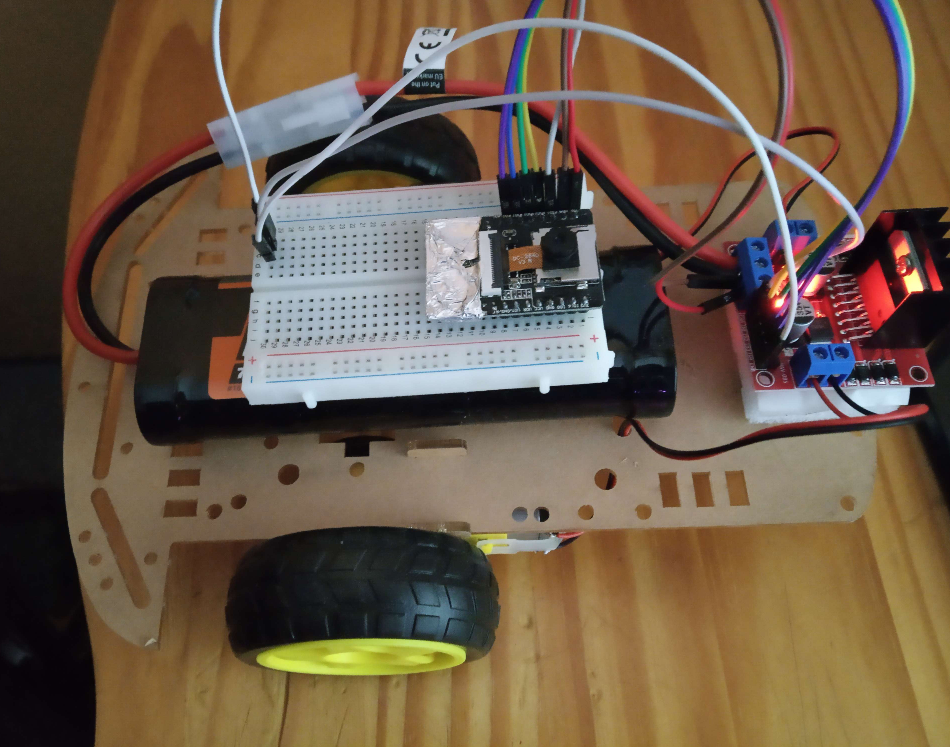
\includegraphics[width=0.65\linewidth]{image/car.png} 
		\end{figure}
		
		\vspace{0.02 \textheight}
		\begin{table}[h!]
			\begin{tabular}{ll}
				\textbf{Autor:} & \jmenoAutora\\ 
				\textbf{Obor:} & \kodOboru { } \obor\\
				\textbf{} & \zamereni\\
				\textbf{Třída:} & \trida\\
				\textbf{Školní rok:} & \skolniRok\\
			\end{tabular}
			
		\end{table}		
	}	
\clearpage
	
%% Stránka obsahující poděkování a prohlášení
%%%%%%%%%%%%%%%%%%%%%%%%%%%%%%%%%%%%%%%%%%%%%%%%%%%%%%%%
%% Poděkování - nepovinné
%%%%%%%%%%%%%%%%%%%%%%%%%%%%
	
	\noindent{\large{\bfseries{Poděkování}\\}}
	\noindent Děkuji panu učiteli Mgr. Marcelu 
Godovskému za jeho doporučení a půjčení testovacích součástek a panu učiteli Mgr. Markovi Lučnému za cené rady s webem.
	
	\vspace*{0.6\textheight} %% Vertikální mezeru je možné upravit

%% Prohlášení - povinné
%%%%%%%%%%%%%%%%%%%%%%%%%%%%
	\noindent{\large{\bfseries{Prohlášení}\\}}  %% uprav si koncovky podle toho na jaký rod se cítíš, vypadá to pak lépe :) 
	\noindent{Prohlašuji, že jsem závěrečnou práci vypracoval samostatně a uvedl veškeré použité 
		informační zdroje.\\}
	\noindent{Souhlasím, aby tato studijní práce byla použita k výukovým a prezentačním účelům na Střední průmyslové a umělecké škole v Opavě, Praskova 399/8.}
	\vfill
	\noindent{V Opavě \datumOdevzdani\\}
	\noindent
	\begin{minipage}{\linewidth}
		\hspace{7.5cm} 
		\begin{tabular}{@{}p{6cm}@{}}
			\dotfill \\
		Podpis autora
		\end{tabular}
	\end{minipage}
	
	\clearpage %% Zalomení

%% Stránka obsahující abstrakt (anotaci)
%%%%%%%%%%%%%%%%%%%%%%%%%%%%%%%%%%%%%%%%%%%%%%%%%%%%%%%%	
	\noindent{\Large{\bfseries{Abstrakt}\\}}
	\noindent Tento projekt se zabývá vytvoření RC auta s využitím vývojové desky ESP32-CAM a Arduina. Komunikace s RC autem probíhá přes WiFi, kde uživatel zadává heslo k připojení. Po úspěšném připojení k síti pomocí mobilu nebo počítače zadává IP adresu, čímž se připojuje na server RC auta. Na obrazovce se okamžitě zobrazuje živý obraz z kamery, spolu s šipkami umožňujícími ovládání pohybu vozidla. Uživatel tak může intuitivně a v reálném čase ovládat RC auto prostřednictvím svého zařízení.
	
	\vspace{18pt}
	
	\noindent{\large{\bfseries{Klíčová slova}}}
	
	\noindent RC auto, ESP32-CAM, Arduino, WiFi, vzdálené ovládání, kamera

    \noindent{\Large{\bfseries{Abstrakt v angličtině}\\}}
    \noindent This project deals with the creation of an RC car using the ESP32-CAM development board and Arduino. Communication with the RC car is via WiFi, where the user enters a password to connect. After successfully connecting to the network using a mobile phone or computer, the user enters an IP address to connect to the RC car server. A live image from the camera is displayed on the screen, along with arrows to control the movement of the vehicle. This allows the user to control the RC car intuitively and in real time with their device.
    
    \clearpage
%% Stránka s generovaným obsahem
%%%%%%%%%%%%%%%%%%%%%%%%%%%%%%%%%%%%%%%	
        \setcounter{tocdepth}{3}  % Zahrnuje subsekce do obsahu
        \setcounter{secnumdepth}{3}  % Čísluje subsekce
        \fancypagestyle{originalplain}{
  \fancyhf{}
  \fancyfoot[C]{\thepage} % Example: put page number at center of footer.
  \renewcommand{\headrulewidth}{0pt}
  \renewcommand{\footrulewidth}{0pt}
}

% Redefine the 'plain' page style to be empty
\fancypagestyle{plain}{
  \fancyhf{} % clear all header and footer fields
  \renewcommand{\headrulewidth}{0pt}
  \renewcommand{\footrulewidth}{0pt}
}
        \tableofcontents %% Vygeneruje tabulku s obsahem
        \clearpage
% Restore the standard 'plain' page style immediately after the ToC
\fancypagestyle{plain}{%
  % Restore the original 'plain' style definitions
  \fancyhf{}
  \fancyfoot[C]{\thepage} % Example: put page number at center of footer.
  \renewcommand{\headrulewidth}{0pt}
  \renewcommand{\footrulewidth}{0pt}
}
% Reset the page style to your preferred style for subsequent pages
\pagestyle{originalplain} % or 'originalplain' if you want to use the saved 'plain' style    
%% Stránka s úvodem - povinná část
%%%%%%%%%%%%%%%%%%%%%%%%%%%%%%%%%%%%%%%
	\chapter*{Úvod}
	\addcontentsline{toc}{chapter}{Úvod}
%Tento příkaz ručně přidává záznam do obsahu.
%První parametr toc označuje, že přidáváme záznam do Table of Contents (obsahu).
%Druhý parametr chapter specifikuje úroveň záznamu. V tomto případě říkáme, že přidávaný záznam má být považován za kapitolu.
%Třetí parametr Úvod je text, který se objeví v obsahu. V tomto případě bude v obsahu zobrazen název "Úvod".
\noindent Od dětství mě fascinovala RC auta. Mým dlouholetým snem bylo sestavit vlastní RC auto a prozkoumat, jak mohu tuto technologii využít. Rozhodl jsem se uskutečnit svou touhu sestavit RC auto s možností ovládání přes WiFi a přenosem obrazu z kamery.

\noindent Cílem tohoto projektu bylo nejen vytvořit plně funkční RC auto, ale také se naučit proces sestavení a zapojení komponent. Klíčovou částí mé práce bylo propojení RC auta s WiFi serverem, což umožňuje vzdálené ovládání a sledování prostřednictvím kamery.

\noindent Během této dokumentace zahrnu sestavení RC auta, implementaci WiFi serveru a integraci kamery. Momentálně auto umožňuje ruční ovládání a sledování terénu. Mým plánem do budoucna je rozšířit funkcionalitu auta o detekci překážek a možnost automatického pohybu. Uvědomuji si, že tato funkce přinese další rozměr a zajímavost do projektu. V závěru se zaměříme na současný stav projektu, popsání dosažených cílů a ohodnocení odvedené práce.

%Tipy k psaní úvodu
%Je povinný, nadpis neměňte, rozsah - max. 1 strana. 
%Tato část práce obsahuje: 
%* náhled do řešené problematiky, zdůvodnění volby problematiky, 
%* předem definované cíle práce, 
%* motivaci pro další čtení textu včetně stručného uvedení obsahu následujících kapitol 

\pagestyle{plain}
\chapter{VÝROBA A SESTAVENÍ RC MODELU}
\noindent Celý proces výroby a sestavování RC modelu započal výběrem vhodných součástek, což pro mě jako nováčka v tomto odvětví zabralo spoustu času. Musel jsem pečlivě vybírat, abych zajistil, že všechny součástky budou vzájemně kompatibilní a celý model bude spolehlivě fungovat.

\noindent Původní plán vytisknout model auta 3D tiskárnou se změnil, když jsem objevil existující model, který nejenže splňoval mé požadavky, ale obsahoval i některé z potřebných součástek. To mi z části ušetřilo čas a zjednodušilo celý proces.

\noindent Sestavování bylo krok po kroku, součástka po součástce. Dával jsem pozor na každý detail, aby vše bylo správně připojeno a pevně drželo. Ostatní součástky jsem testoval předtím, než jsem je úplně zapojil, abych se vyhnul pozdějším potížím.

\noindent Až poté, co bylo vše fyzicky spojeno, přišla na řadu fáze programování. Začal jsem s jednoduchými příklady pro zobrazení obrazu z kamery. Pro programování jsem použil jazyk Arduino, což je kombinace jazyku C a C++. Na komunikaci s webem jsem potřeboval speciální balíčky, například AsyncTCP, který tvořil základ pro ESPAsyncWebServer. Design webového rozhraní jsem upravil s pomocí HTML, CSS a dalších technologií, které mi ulehčili zpříjemnit vzhled stránky.
\newpage
\section{Použitý hardware}
\subsection{Seznam součástek}
\begin{itemize}
    \item Vývojová deska ESP32-CAM,
    \item H můstek L298N Dual H Most DC,
    \item Arduino MEGA 2560 Rev3,
    \item Hadex motorek 3-6V/0,17A s převodovkou, převod 1/48
    \item akumulátor HPI Plazma Ni-MH 7.2V 2000mAh 
    \item snímač otáček
    \item nepájivé pole
\end{itemize}

\subsection{ESP32-CAM}
\noindent Základem mého projektu byla vývojová deska ESP32-CAM (obrázek č. 1). Poskytla mi opravdu skvělý způsob jak přidat vizuální prvek do mého projektu. Tato deska spojuje výkonný mikrokontrolér ESP32 s kamerovým modulem, což umožňuje snadné zachycení a zpracování obrazu. Díky flexibilním GPIO pinům, podpoře pro paměťové karty a jednoduchému programování pomocí Arduino IDE poskytuje ideální řešení pro mé potřeby. S integrovanou WiFi podporou je snadné přenášet data bezdrátově, což rozšiřuje možnosti komunikace a přenosu informací.
\begin{figure}[h]
    \begin{subfigure}{0.48\textwidth}
        \centering
		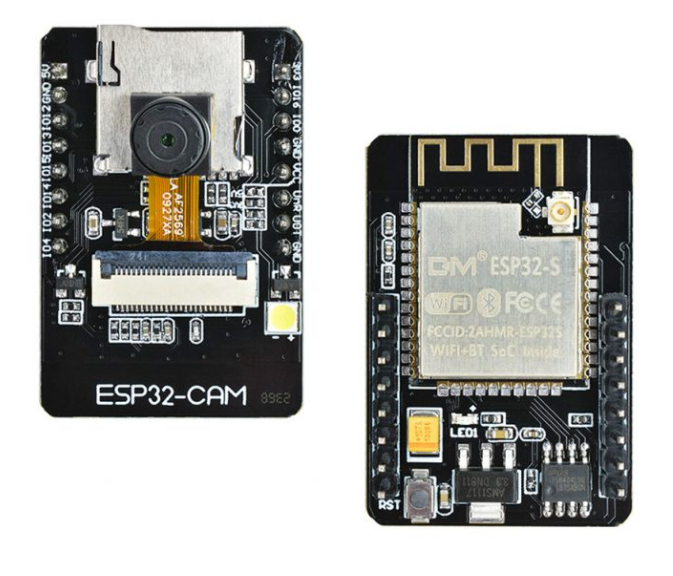
\includegraphics[width=\textwidth]{image/esp32.png}
        \caption*{\textit{obrázek č. 1 ESP32-CAM}}
        \label{fig:esp32}
    \end{subfigure}
    \begin{subfigure}{0.48\textwidth}
        \centering
        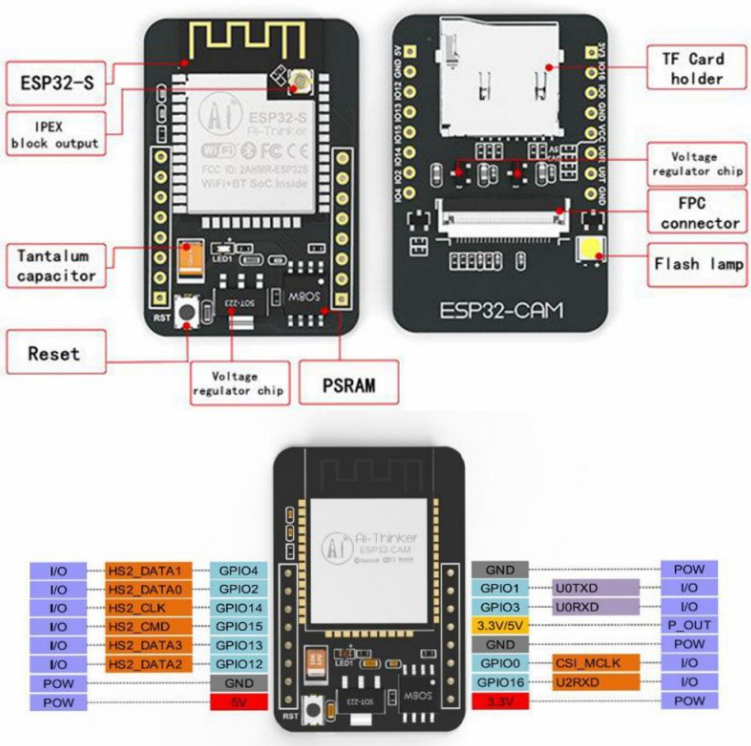
\includegraphics[width=\textwidth]{image/esp32-pins.png}
        \caption*{\textit{obrázek č. 2 Piny ESP32-CAM}}
        \label{fig:esp32Pins}
    \end{subfigure}     
\end{figure}

\subsection{L298N Dual H Most DC}
    \noindent V rámci mého projektu RC auta se H-můstek L298N (obrázek č. 3) stal důležitou součástí pro pohyb DC motorů. Jeho snadné zapojení a schopnost nezávislého ovládání obou motorů dodaly projektu potřebnou variabilitu pro dosažení plynulého pohybu vozidla.

    \noindent Během integrování H-můstku L298N do celkového systému jsem ocenil jeho přehledný design a spolehlivost. Jeho spolupráce s mikrokontrolérem umožnila programovat pohyb motorů tak, jak jsem si představoval. Vyzkoušel jsem i možnosti stanovení rychlosti motorů.
    \begin{figure}[H]
        \centering
		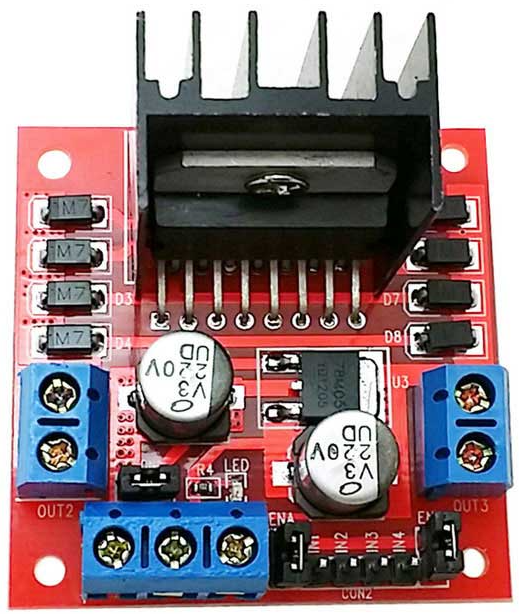
\includegraphics[width=0.35\textwidth, height=4.5cm]{image/Hmustek.png}
        \caption*{\textit{obrázek č. 3 L298N Dual H Most DC}}
        \label{fig:hMustek}
    \end{figure}

\subsection{Arduino MEGA 2560 Rev3}
\noindent Původně jsem plánoval využít Arduino MEGA 2560 Rev3 jako hlavní řídící jednotku pro mé RC auto. Nicméně, během průběhu projektu jsem se rozhodl pro interaktivnější přístup a zvolil jsem ESP32-CAM. Arduino MEGA 2560 Rev3 jsem nakonec využil pouze jako programátor pro nahrávání kódu do ESP32-CAM. Jeho schopnosti, jako bohatý počet digitálních a analogových pinů (obrázek č. 4), spolu s rozsáhlou pamětí, mi poskytly spolehlivý nástroj pro efektivní práci s ESP32-CAM a programování v Arduino IDE.
\begin{figure}[H]
        \centering
		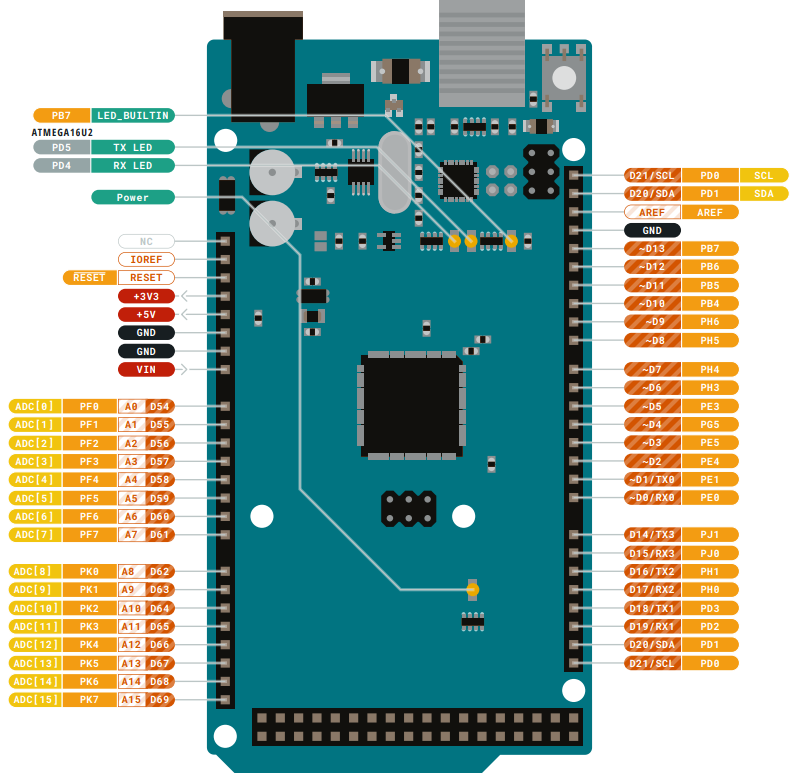
\includegraphics[width=0.48\textwidth]{image/arduionoPins.png}
        \caption*{\textit{obrázek č. 4 Piny Arduino MEGA }}
        \label{fig:arduino}
    \end{figure}

\subsection{Hadex motorek 3-6V/0,17A}
\noindent Pro pohyb mého RC auta jsem se rozhodl využít Hadex motorek 3-6V/0,17A s převodovkou. Tyto motorky nabízejí optimální kombinaci výkonu a efektivity, ideální pro plynulý pohyb vozidla. S napětím 3-6V a proudem 0,17A poskytují spolehlivý výkon. Převodovka s poměrem 1/48 přináší možnost jemného nastavení rychlosti a výkonu.

\subsection{HPI Plazma Ni-MH 7,2V 2000mAh}
\noindent Posledním kouskem mého RC auta byl pečlivě vybraný akumulátor HPI Plazma 2000mAh NiMH 7,2V (obrázek č. 5). S kapacitou 2000mAh poskytuje dlouhý provoz. Je ideální pro rozsáhlé závody nebo delší dojížďky. Jeho technologie NiMH zajišťuje spolehlivý pohon motorů a odolný design je připraven i na náročnější terény. Hlavně tato baterie dodává mému RC autu potřebnou energii pro maximální výkon.
\begin{figure}[H]
        \centering
		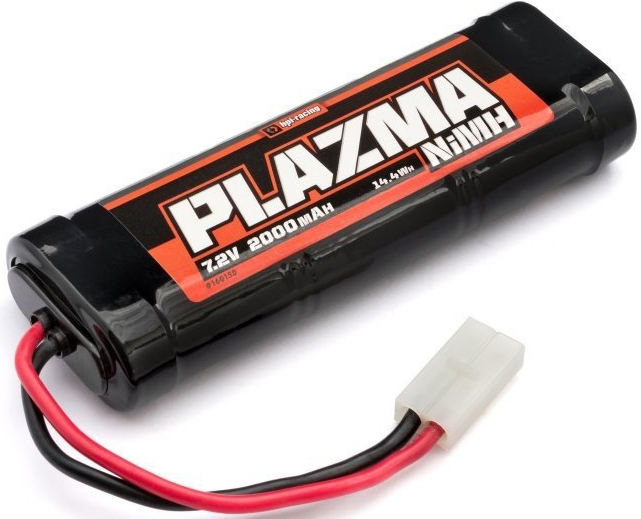
\includegraphics[width=0.48\textwidth]{image/akumulator.png}
        \caption*{\textit{obrázek č. 5 HPI Plazma Ni-MH 7,2V 2000mAh}}
        \label{fig:akumulator}
    \end{figure}

\section{Použitý software}
\subsection{Použitý jazyk}
\noindent Pro mé RC auto jsem použil programovací jazyk Arduino, který nabízí efektivní a snadný způsob psaní kódu pro mikrokontroléry. Jazyk Arduino vychází z C a C++, ale je přizpůsoben pro jednoduchost a srozumitelnost i pro začátečníky v programování. Díky své intuitivní syntaxi a podpoře komunity se stal nepostradatelným nástrojem pro vytváření elektronických projektů.

\subsection{Arduino IDE}
\noindent Pro psání kódu jsem využil vývojové prostředí Arduino IDE 2.2.2 bylo pro můj projekt klíčové. Jeho integrovaný editor kódu, podporující automatické doplňování, výrazně usnadnil psaní kódu. Toto užitečné funkce nejen zvýšily efektivitu mé práce, ale také minimalizovaly chyby v kódu. 

\newpage
\subsection{Web Server}
\noindent Využil jsem knihovnu ESPAsyncWebServer pro implementaci WebServeru na mikrokontrolér ESP32. Tato knihovna poskytuje asynchronní zpracování webových požadavků. Pro zlepšení rozhraní jsem využil moderní webové technologie, včetně HTML, CSS a JavaScriptu. Na stránce jsou tlačítka pro ovládání pohybu vozidla a posuvník pro nastavení intenzity světela.

\subsection{WebSocket komunikace}
\noindent V projektu jsem využil WebSocket komunikaci s knihovnou ESPAsyncWebServer, což umožnilo rychlou a efektivní výměnu dat mezi mikrokontrolérem a webovým rozhraním. K posílání funkcí a interaktivnímu ovládání na straně webového rozhraní jsem implementoval JavaScript, což poskytuje uživatelům schopnost aktivně ovládat a komunikovat s mikrokontrolérem přes webové rozhraní.

\chapter{PRINCIP VZDÁLENÉHO OVLÁDÁNÍ}
\noindent Mým primárním cílem bylo navázat bezdrátovou komunikaci prostřednictvím WiFi. K tomu jsem využil mikrokontrolér ESP32 a Arduino, kde Arduino plnilo roli programátoru pro nahrávání kódu do ESP32. Zásadním krokem bylo vytvoření spojení se serverem. Ovladač (mobilní zařízení nebo počítač) se připojí k serveru přes WiFi po zadání přístupových údajů (hesla) se naváže spojení umožňující zadat IP adresu do prohlížece a zahájit komunikaci mezi ovladačem a modelem RC auta.

\noindent Implementace ovládání vozidla byla následným krokem, kde na webovém rozhraní byla integrována šipková tlačítka umožňující pohyb vozidla vpřed, vzad, doprava a doleva. To vytvořilo intuitivní a snadno ovladatelný systém.





\chapter{POUŽITÉ POSTUPY A ŘEŠENÍ}

\section{HARDWARE TECHNOLOGIE}

\subsection{Schéma}
\noindent Jako první jsem se zaměřil na propojení motorů s H-můstkem pro ovládání pohybu. Každý motor byl připojen k určeným pinům pro otáčení vzad a vpřed. Kamera ESP32-CAM byla také integrována do H-můstku, ale bylo třeba upravit některé kabely kvůli optimálnímu propojení, zejména v oblasti spojení s GND, kde jsem potřeboval zapojit i GND z baterie. Abych zajistil správné napájení kamery, použil jsem zdroj proudu z baterie s napětím 7,2 V, následně jsem snížil napětí na 5 V pro kameru pomocí pinu na H-můstku. 
\begin{figure}[H]
        \centering
		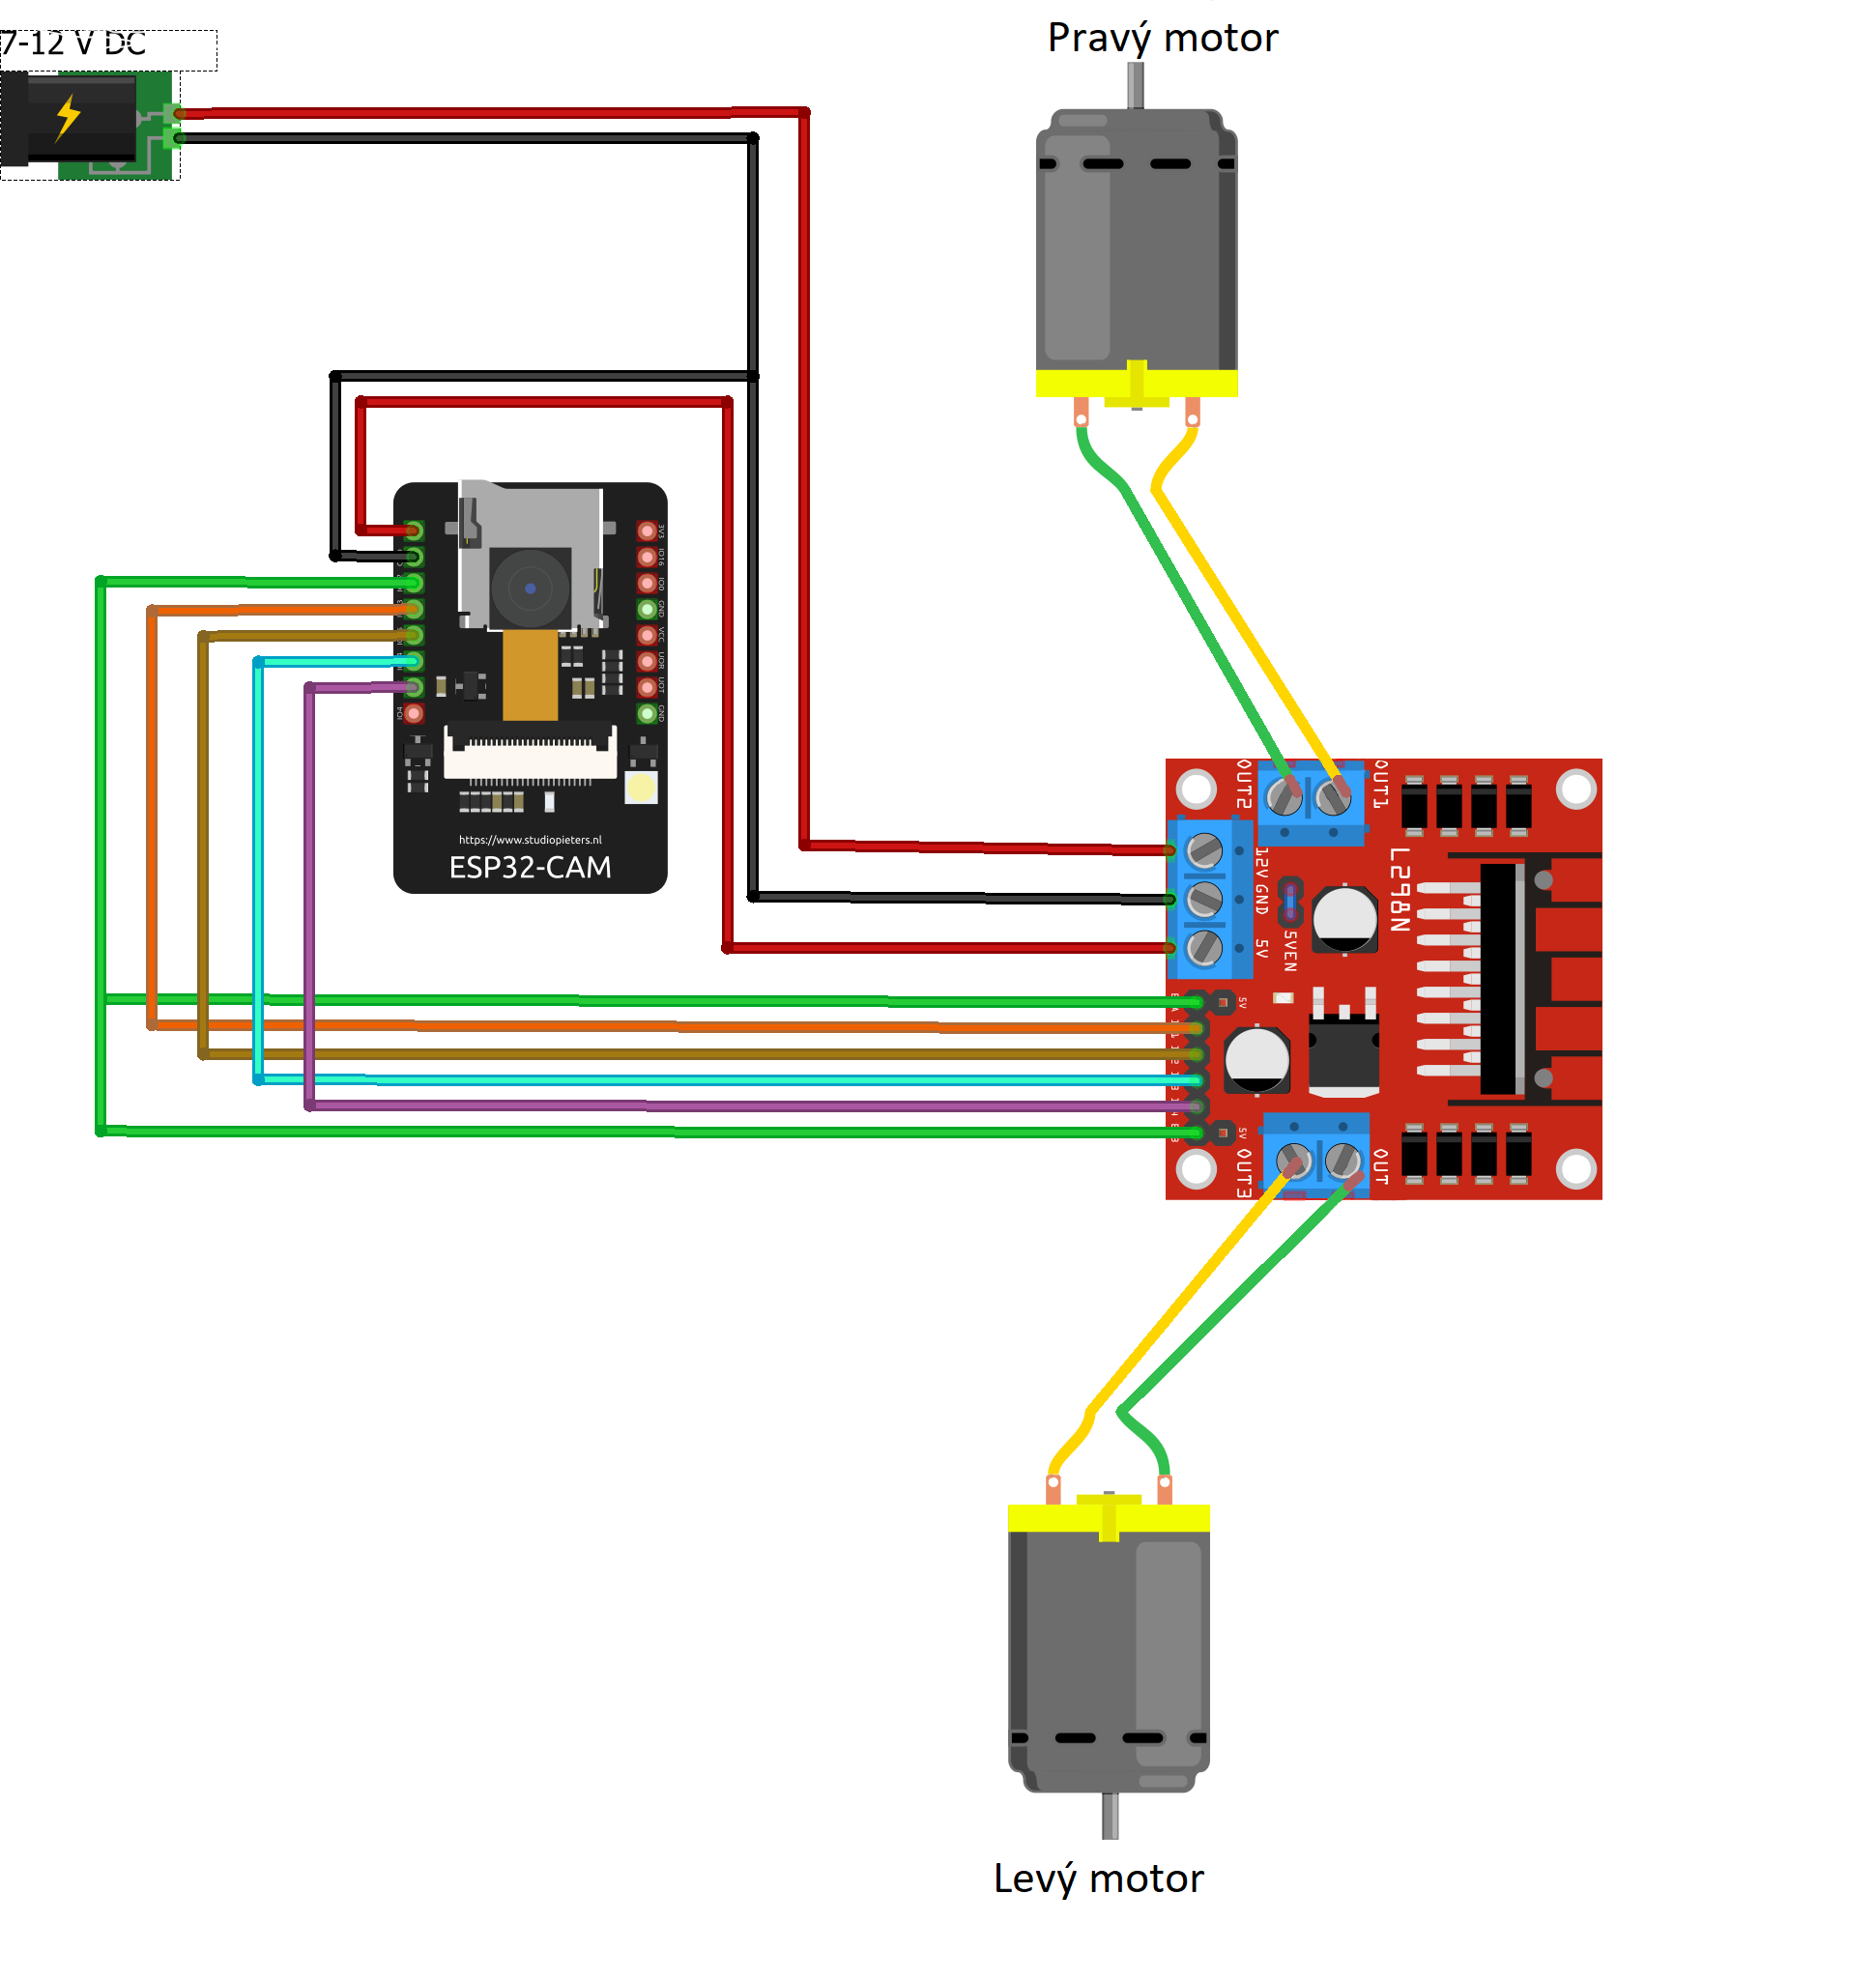
\includegraphics[width=0.6\textwidth]{image/schema.png}
        \caption*{\textit{obrázek č. 6 Schéma}}
        \label{fig:shema}
    \end{figure}
    
\subsection{Nahrávání kódu}
\noindent Během nahrávání kódu do ESP32-CAM jsem využíval Arduino Mega jako programátor. Pro tento účel bylo zapotřebí specifického zapojení (viz obrázek č. 7), přičemž každý nahrávací cyklus vyžadoval ruční reset ESP32-CAM ze zadní strany. Tento postup však značně zpomaloval celý proces. Mým doporučením je použití ESP32-CAM-MB, i když v mém konkrétním projektu jsem tento modul bohužel nenasadil.
\begin{figure}[h]
    \begin{subfigure}{0.48\textwidth}
        \centering
		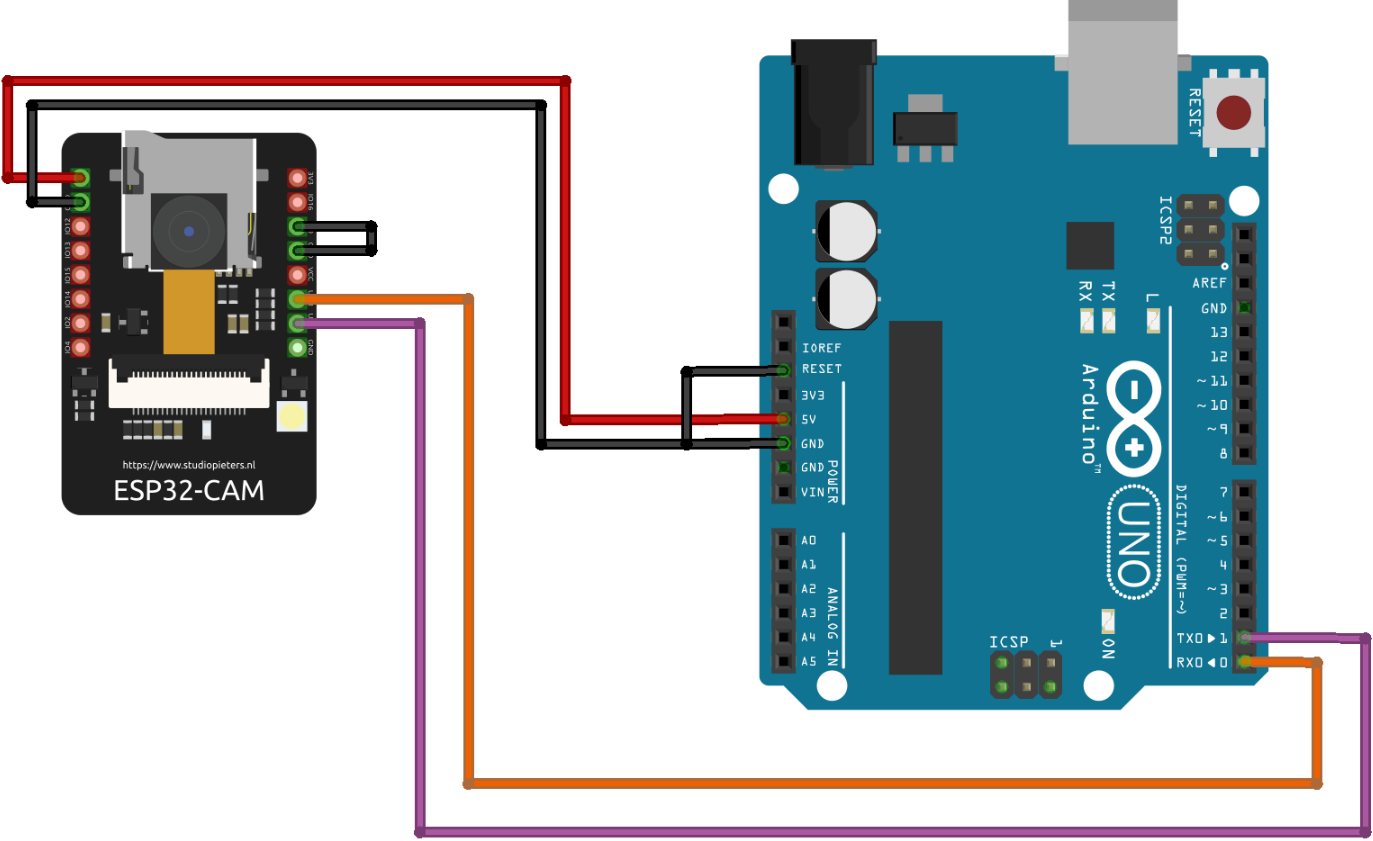
\includegraphics[width=\textwidth]{image/schemaNahrani.png}
        \caption*{\textit{obrázek č. 7 Schéma arduiono a esp32-cam}}
        \label{fig:schemaArduino}
    \end{subfigure}
    \begin{subfigure}{0.48\textwidth}
        \centering
        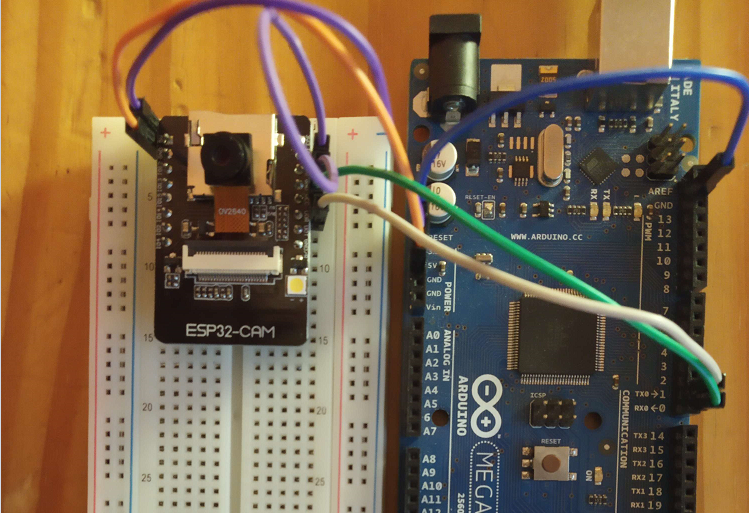
\includegraphics[width=\textwidth]{image/nahravaniVPraxi.png}
        \caption*{\textit{obrázek č. 8 Ukazka nahravani v praxi}}
        \label{fig:nahraniVPraxi}
    \end{subfigure}     
\end{figure}

\subsection{Definice proměných a knihoven}
\noindent Pro ovládání motorů jsem vytvořil strukturu MOTOR PINS a v ní definovat vektor motorPins, který obsahuje informace o pinech pro každý motor. Pomocí PWM signálu mám možnost plynule upravovat rychlost motorů podle potřeby. Abych dosáhl optimálního řízení, nastavil jsem konstanty pro frekvenci (PWMFreq) a rozlišení (PWMResolution) PWM signálu. Dále jsem provedl inicializaci pinů sloužících k řízení rychlosti motorů a přiřadil je k odpovídajícím PWM kanálům.
\subsection{Řešení ovládání vozidla}
\noindent Ovládání pohybu vozidla jsem implementoval pomocí dvou funkcí. První z nich, rotateMotor(), umožňuje kontrolu otáčení motorů podle zadaného směru. Využívá předem definovanou strukturu MOTOR PINS a vektor motorPins, který obsahuje informace o pinech pro každý motor.
\begin{lstlisting}[caption={Příklad funkce moveCar()}, label=lst:arduino]
void moveCar(int inputValue) {
  Serial.printf("Got value as %d\n", inputValue);
  switch (inputValue) {
    case UP:
      rotateMotor(RIGHT_MOTOR, FORWARD);
      rotateMotor(LEFT_MOTOR, FORWARD);
      break;
    case DOWN:
      rotateMotor(RIGHT_MOTOR, BACKWARD);
      rotateMotor(LEFT_MOTOR, BACKWARD);
      break;
    case LEFT:
      rotateMotor(RIGHT_MOTOR, FORWARD);
      rotateMotor(LEFT_MOTOR, BACKWARD);
      break;
    case RIGHT:
      rotateMotor(RIGHT_MOTOR, BACKWARD);
      rotateMotor(LEFT_MOTOR, FORWARD);
      break;
    case STOP:
      rotateMotor(RIGHT_MOTOR, STOP);
      rotateMotor(LEFT_MOTOR, STOP);
      break;
    default:
      rotateMotor(RIGHT_MOTOR, STOP);
      rotateMotor(LEFT_MOTOR, STOP);
      break;
  }
}
\end{lstlisting}
\newpage
\noindent Druhou funkcí je moveCar(), která přebírá vstupní hodnotu a na základě ní řídí pohyb vozidla. Používá funkci rotateMotor pro nastavení různých směrů pohybu, jako jsou nahoru, dolů, doleva a doprava. Při příjmu hodnoty UP nebo DOWN jsou oba motory nastaveny tak, aby se vozidlo pohybovalo vpřed nebo vzad. Při směrech LEFT a RIGHT jsou motory nakonfigurovány tak, aby vozidlo rotujícím způsobem změnilo směr.

\section{Web server}
\subsection{Zpracování dat}
\noindent V další části kódu se starám o komunikaci mezi webovým rozhraním a vozidlem. Funkce onCarInputWebSocketEvent() je vyvolána při různých událostech spojených s WebSocket. Když se klient připojí, ukládají se informace o připojení. Pokud klient odejde, zastaví se pohyb vozidla a vypne se světlo. Funkce initCarInputWebSocket() inicializuje WebSocket pro příjem ovládacích příkazů od klienta. Při připojení klienta jsou automaticky nastaveny výchozí hodnoty rychlosti a světla vozidla. Ve smyčce loop() neustále komunikuji přes WebSocket a čistím nepoužívané klienty. Ovládání vozidla je obsaženo ve funkci moveCar(), kde jsou na základě příchozích hodnot řízeny pohyby vozidla.
\begin{lstlisting}[caption={Ukázka zpracování odpojení a připojení klienta}, label=lst:arduino]
void onCarInputWebSocketEvent(AsyncWebSocket *server,
                              AsyncWebSocketClient *client,
                              AwsEventType type,
                              void *arg,
                              uint8_t *data,
                              size_t len) {
  switch (type) {
    case WS_EVT_CONNECT:
      Serial.printf("WebSocket client #%u connected from %s\n", client->id(), client->remoteIP().toString().c_str());
      break;
    case WS_EVT_DISCONNECT:
      Serial.printf("WebSocket client #%u disconnected\n", client->id());
      moveCar(0);
      ledcWrite(PWMLightChannel, 0);
      break;
\end{lstlisting}
\subsection{Vzhled}
\noindent Webové rozhraní obsahuje obrazový prvek pro zobrazení kamery a tlačítka pro ovládání vozidla, umístěná uvnitř kontejneru. Rozhraní je stylizováno pomocí CSS, které zajištujě reponzivitu. Pro ovládání pohybu vozidla jsou k dispozici čtyři tlačítka (nahoru, dolů, doleva, doprava), která jsou implementována jako HTML tlačítka s ikonami SVG. Každé tlačítko reaguje na interakci s myší nebo dotykem na dotykovém zařízení. Kromě ovládání pohybu vozidla jsou k dispozici další prvky, jako posuvník pro nastavení intenzity světla na vozidle.

	\chapter{Výsledky řešení}

    \section{Podoba RC auta}
    \noindent RC auto momentálně představuje funkční jednotku s minimalistickým vzhledem. Pro dosažení esteticky poutavější podoby a zároveň zvýšení odolnosti plánuji přidat karosérii. Aktuálně je vozidlo křehké. To chci vyřešit přidáním karosérie. Do budoucna mám v úmyslu lépe organizovat součástky tak, aby se snadněji aplikovala karosérie. Toto uspořádání by mělo zohledňovat nejen estetiku, ale také praktičnost údržby. Také bych chtěl optimalizovat rozmístění drátků, které v současné době občas mohou narušit chod auta a vadit objektivu kamery. Mým cílem je zajistit bezproblémový provoz a zvýšit celkovou spolehlivost RC auta.
       \begin{figure}[H]
    \centering
	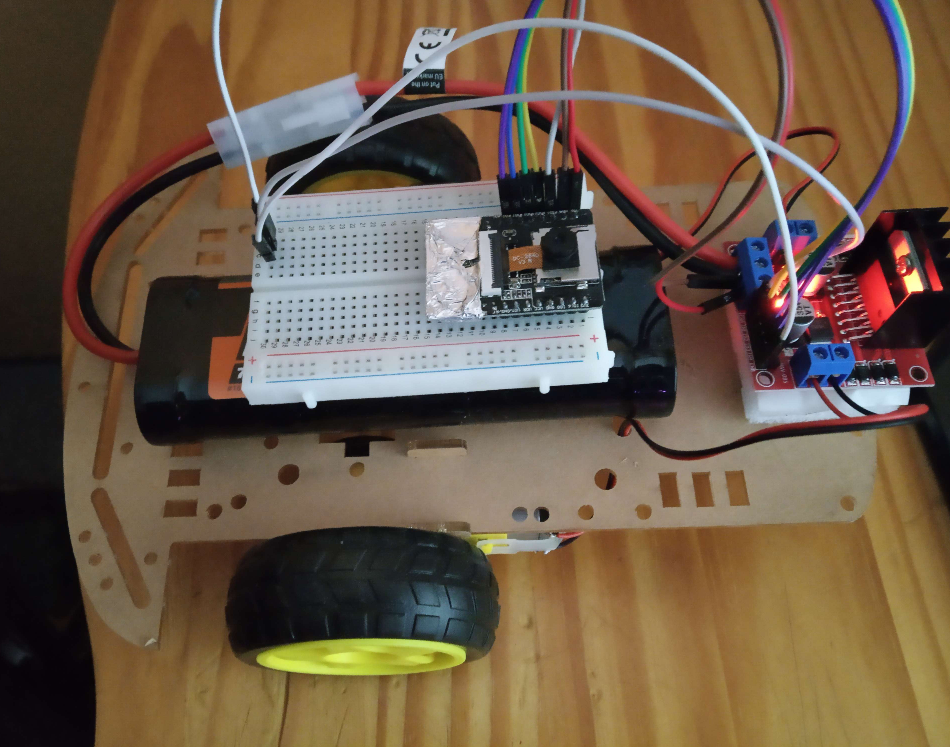
\includegraphics[width=0.8\textwidth]{image/car.png}
    \caption*{\textit{obrázek č. 9 Vzhled auta}}
    \label{fig:webDesign}
\end{figure}
    
    \section{Podoba klienta}

    \noindent Web server splňuje svůj účel, umožňuje snadné ovládání mého RC auta. Připojení k serveru je jednoduché - stačí se připojit k WiFi pomocí hesla a zadat správnou IP adresu do vyhledávače. Ihned se ocitneme v interaktivním rozhraní. Současný design webové stránky zaručuje plnou responzivitu, což umožňuje pohodlný přístup nejen z počítačů, ale také z mobilních zařízení. Díky integrované kameře máme možnost sledovat skutečný obraz z kamery.
    \begin{figure}[H]
    \centering
	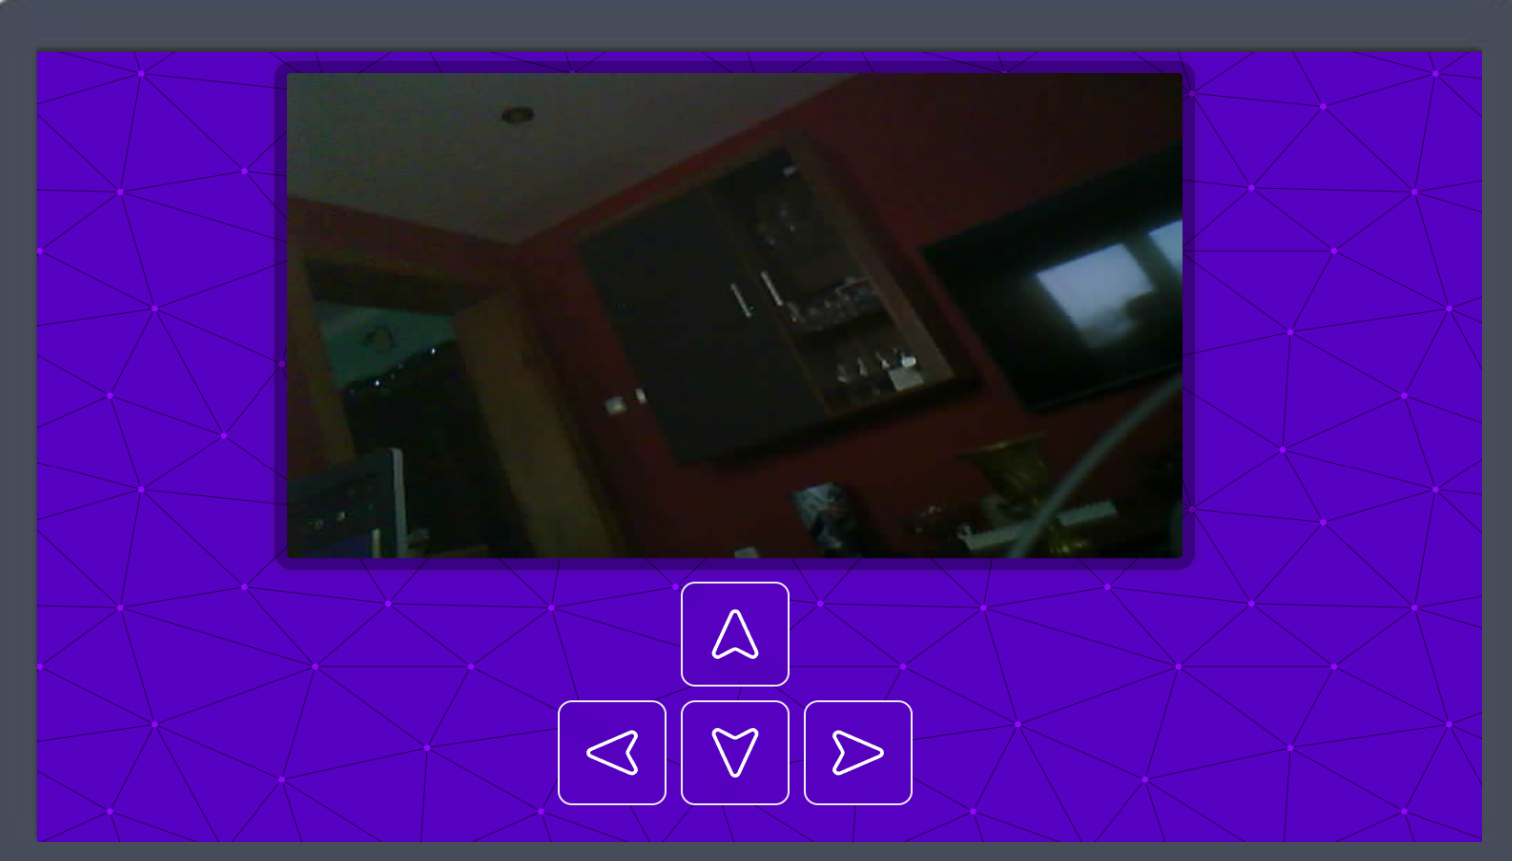
\includegraphics[width=0.9\textwidth]{image/web.png}
    \caption*{\textit{obrázek č. 10 Jednoduchá ukázka webu bez obrazu kamery}}
    \label{fig:webDesign}
\end{figure}
 
	\chapter*{Závěr}
	\noindent Hlavní cíle mého projektu zahrnovaly sestavení funkčního RC auta, jeho dálkové ovládání přes WiFi a přenos obrazu z kamery. Zadané cíle byly s úspěchem dosaženy. RC auto bylo úspěšně sestaveno a vybaveno funkcemi dálkového ovládání a přenosu obrazu z kamery. I když se v průběhu projektu objevily další nápady, jako je detekce překážek a automatický pohyb, ty jsou plánovány pro budoucí vylepšení. Rovněž se zamýšlím nad vylepšením vizuálního designu auta, ale nepodařilo se mi aplikovat plánovaný model. Projekt byl pro mě inspirativní a přinesl spoustu výzev, ačkoli ne všechny části byly dokončeny podle původního plánu.

    \noindent Odkaz na GitHub: \href{https://github.com/MichaelMeinhard/zaverecny-projekt}{https://github.com/MichaelMeinhard/zaverecny-projekt}
	
	%% literatura
	\begin{thebibliography}{99}
		\bibitem{sspuLogo} \textit{Střední škola průmyslová a umělecká Opava} [online]. [cit. 2023-11-11]. Dostupné z: \url{https://www.sspu-opava.cz}
        \bibitem{esp32Cam} \textit{Drátek} [online]. [cit. 2023-28-12].
        Dostupné z: \url{https://dratek.cz/arduino/7587-esp32-cam-vyvojova-deska-wifi-bluetooth-s-kamerovym-modulem-ov2640.html}
        \bibitem{HMustek} \textit{Drátek} [online]. [cit. 2023-28-12].
        Dostupné z: \url{https://dratek.cz/arduino/877-arduino-h-mustek-pro-krokovy-motor-l298n-dual-h-most-dc.html}
        \bibitem{arduinoMega} \textit{Arduino docs} [online]. [cit. 2023-28-12].
        Dostupné z: \url{https://docs.arduino.cc/hardware/mega-2560l}
        \bibitem{akumulátor} \textit{Mz racing} [online]. [cit. 2023-28-12].
        Dostupné z: \url{https://www.mz-racing.net/160150-hpi-plazma-2000mah-nimh-7-2v-p42595}
	\end{thebibliography}	
\end{document}